Let
\begin{align}
\vec{P} = \myvec{0\\0}, \vec{Q} = \myvec{4\\0}, \vec{R} = PR\myvec{\cos \theta\\  \sin \theta}
\end{align}
where,
\begin{align}
    PR\brak{\frac{\sin\theta}{2}}&=\frac{QR}{2}
    \\
    \implies \theta &=2\sin^{-1}\brak{\frac{QR}{2PR}}
\\
  &=51.88
\end{align}
% \begin{align}
%     \vec{R}=\myvec{2.47\\3.15}
%     \end{align}
Thus, the vertices of $\triangle PQR$ are
\begin{align}
\vec{P} = \myvec{0\\0}, \vec{Q} = \myvec{4\\0}, \vec{R} = \myvec{2.47\\3.15}
\end{align}
% Lines $PQ$ ,$QR$ and $RP$ are then generated and
% plotted using these coordinates to form $\triangle PQR$

% Here
% In $\triangle PQR$ Two sides are equal.
% So $\triangle PQR$ is a isosceles triangle.

which are used to plot  $\triangle PQR$  in Fig. \ref{constr/tri/12fig:isosceles_triangle}.	
%
\begin{figure}[!ht]
\centering
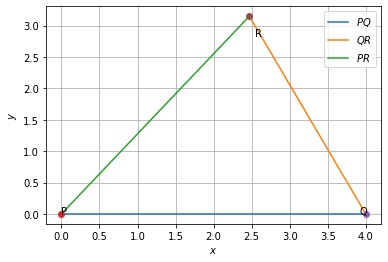
\includegraphics[width=\columnwidth]{solutions/triangle/12/fig.png}
\caption{isosceles $\triangle PQR$}
\label{constr/tri/12fig:isosceles_triangle}	
\end{figure}

